% Author: Daniel Celis Garza <daniel.celisgarza@materials.ox.ac.uk>
% Date of creation: 2017/03/09
% Last edit: 2017/03/09

% Preamble with all the basic packages a thesis would need. Modify as needed.

\documentclass[htwologo,twosup,12pt]{genthesis}
% By changing the document class this preamble can be used for other document types.
% genthesis.cls contains the definition of the document class.
% Geometry
\usepackage[top=1in, bottom=1in, 
			outer=1in, inner=1in] % inner = 1.5 for binding
			{geometry}

%----------------------- Fonts, symbols and colours ------------------------%
% If using pdfLaTeX comment fontspec and uncomment fontenc and inputenc. If using the superior XeLaTeX/XeTeX or LuaTeX do the opposite.
\usepackage{fontspec}					% XeLaTeX & LuaTeX fonts.
%\usepackage[T1]{fontenc}				% Font encoding for pdfLaTeX
%\usepackage[latin1]{inputenc}			% Input encoding (easy accents) for pdfLaTeX
\usepackage{amssymb, amsmath,
			bm	   , isomath,
			mathtools}					% Maths fonts and symbols.
\usepackage{exscale}					% Removes the need to use {\displaystyle }.
%\newfontfamily\ubuntumono{Ubuntu Mono} % Ubuntu font for fancy shell commands (font needs to be installed).
\usepackage{xcolor}
%\definecolor{oxfordblue}{cmyk}{79,56,0,72}
\definecolor{oxfordblue}{RGB}{15,31,71}
\usepackage{lmodern}

%------------------------ Hyperlinks and references ------------------------%
\usepackage[colorlinks     = true, % Hyperlinks.
			pdfstartview   = FitV,
			linkcolor      = oxfordblue,
			citecolor      = oxfordblue,
			urlcolor       = oxfordblue,
			hyperfootnotes = true,
			hypertexnames  = true,
			plainpages     = false % Correctly links index entries whenever \thispagestyle{empty} is used.
			]{hyperref}
\usepackage[comma  , square,       % Citing style.
			numbers, sort&compress
			]{natbib}
\usepackage{cleveref} 			   % Automatic referencing better than \autoref{}.

%--------------------------- Index and glossary ----------------------------%
\usepackage{makeidx} % Index.
\usepackage{xparse}	 % Expanded macro capability.
\makeindex			 % Creates index.
\usepackage[toc, acronyms
			]{glossaries} % Glossary.
\setglossarystyle{altlisthypergroup} % Sets a list of letters with hyperlinks before the glossaries and acronyms.
% Dual glossary entry.
% Define dual entry for glossary + acronym.
% https://en.wikibooks.org/wiki/LaTeX/Glossary#Dual_entries_with_reference_to_a_glossary_entry_from_an_acronym
\DeclareDocumentCommand{\newdualentry}{ O{} O{} m m m m } {
	\newglossaryentry{gls-#3}{name={#5},text={#5\glsadd{#3}},
		description={#6},#1
	}
	\makeglossaries
	\newacronym[see={[Glossary:]{gls-#3}},#2]{#3}{#4}{#5\glsadd{gls-#3}}
}

%--------------------------------- Utility ---------------------------------%
\usepackage{setspace}  % Text spacing commands.
%\usepackage{paralist} % In-paragraph lists.
%\usepackage{pdfpages} % Include pdf pages.
%\usepackage{lscape}   % Use landscape pages.
%\allowdisplaybreaks   % Math environments continue onto the next page if they overflow.
\usepackage{siunitx}   % International units.
\usepackage{hologo}    % XeLaTeX and BibTex logos.

%--------------------------------- Floats ----------------------------------%
%\usepackage{float} 			% Extra options for floats.
%\usepackage[section]{placeins} % Force floats to stay in the sections they're called in.
\usepackage{booktabs} 			% Nicer tables.
%\usepackage{multirow} 			% Multirow and multicolumn tables. Avoid when possible.
\usepackage{subcaption} 		% Subfigures.
%\usepackage{epstopdf} 			% pdfLaTeX does not support eps images so they need to be converted to pdf.

%---------------------------- Scripts and code -----------------------------%
% If you only need basic script support use verbatim. If you want more features use listings. If you can install pygments use minted.
%\usepackage{verbatim} % Type commands without the hassle of the other two.
%\usepackage{listings} % Spartan display of code and pseudo code.
\usepackage{minted}   % Elegantly display code. Requires a Python 2.7 or higher installation of pygments to be installed. Requires "-shell-escape" flag to the LaTeX compilation command.
\usepackage[chapter]{algorithm}
\usepackage{algpseudocode} % Package for algorithm typesetting (pseudo-code).

%---------------------------- Image file paths -----------------------------%
\graphicspath{{./images/}}

%------------------------------- Input files -------------------------------%
\renewcommand{\vec}{\vectorsym}
\newcommand{\tns}{\tensorsym}
\newcommand{\mtx}{\mathbf}
\newcommand{\hvar}[1]{\ensuremath{^{\textrm{h}}#1}}
\newcommand{\dvar}[1]{\ensuremath{^{\textrm{d}}#1}}
\newcommand{\tvar}[1]{\ensuremath{^{\textrm{t}}#1}}
\newcommand{\rvar}[1]{\ensuremath{\textrm{#1}}}
\newcommand{\nn}{\nonumber\\}							% No number skip line.
\algblockdefx[gpufunction]{GPUFunction}{EndGPUFunction}%
[2][]{\textbf{GPU function} \textsc{#1}(#2)}%
{\textbf{end GPU function}}	 % Macros.
% Entries without acronyms
\newglossaryentry{bv}
{
	name={Burgers vector},
	description={Denoted as $\vec{b}$, it represents the lattice distortion caused by a \kwd{dl} in a crystal lattice. In \emph{edge} \kwdp{dl} the Burgers vector is perpendicular to the line direction ($ \vec{b} \perp t $); in \emph{screw} \kwdp{dl} it is parallel to the line direction ($ \vec{b} \parallel t $); in \emph{mixed} \kwdp{dl}, Burgers vector and line direction are neither perpendicular nor parallel to each other},
	symbol = {\ensuremath{\vec{b}}}
}

\newglossaryentry{dl}
{
	name={dislocation},
	description={Crystallographic defect which strongly influences many of a material's properties. It can consist of additional or missing partial crystallographic planes, and may come in three varieties: edge, screw and mixed. Mathematically it is a type of topological defect/soliton because it is a distinct, out of equillibrium---but stable---solution of the \kwd{pde} which in the trivial case yields the crystallographic structure of a material. Like any other soliton, it will not spontaneously decay to the ``trivial'' solution, which in this case would be a perfect crystal. Thus a dislocation preserves its identity by preserving its \kwd{bv}. Like other solitons, it can annihilate with another of opposite phase, which in this case would be an opposite \kwd{bv}}
}

\newglossaryentry{devmem}
{
	name = {device memory},
	description = {Graphics card memory visible only within GPU functions}
}

\newglossaryentry{atop}
{
	name = {atomic operation},
	description = {An operation on shared or global \kwd{devmem} which is guaranteed to be performed without interference from other threads. However, atomic operations don't act as memory fences and do not imply \kwd{thrsync} \cite{nvidia_atomics}}
}

\newglossaryentry{thrsync}
{
	name = {thread syncronisation},
	description = {Ensures all threads catch up to each other in some way or another. The function \mintinline{c}{__syncthreads()} ensures all threads in a \kwd{wrp} reach the same point. The function \mintinline{c}{__threadfence()} flushes all global memory and shared memory writes by a thread so the updated values are visible to other threads before continuing}
}

\newglossaryentry{cma}
{
	name = {coalesced memory access},
	description = {When all active threads in a \kwd{wrp} access contiguous global memory. Therefore cache lines can be very efficiently utilised}
}

\newglossaryentry{wrp}
{
	name = {warp},
	description = {Collection of threads with a maximum of 32 which execute concurrently on the same \kwd{sm} resources}
}

\newglossaryentry{wrpd}
{
	name = {warp divergence},
	description = {Due to the fact that all threads in a \kwd{wrp} must execute the same instruction concurrently, all program branches are executed regardless of branching condition. However, only those instructions for which a branching condition is met have an effect on the state of the thread's program. As a consequence, different threads in a \kwd{wrp} may meet different branching conditions, wasting all other branched instructions}
}

\newglossaryentry{tensor}
{
	name = {tensor},
	description = {Geometric object that represents linear relations between matrices, vectors, scalars and other tensors}
}

\newglossaryentry{dls}
{
	name = {dislocation line segment},
	description = {Discretisation of dislocations as straight line segments between two tracked nodes},
	plural={dislocation line segments}
}

% Entries with acronyms
% Syntax: \newdualentry[glossary options][acronym options]{label}{abbrv}{long}{description}
\newdualentry
{sm}
{SM}
{Streaming Multiprocessor}
{A differential equation which contains unkown multivariate functions and their partial derivatives. Solutions require knowledge of the boundary conditions the unkown functions are subject to. The types of PDEs and their boundary conditions can make it difficult or impossible to find well-behaved, analytical solutions. As a result, numerical methods such as \kwd{fem} are often used to solve them}

\newdualentry
{pde}
{PDE}
{Partial Differential Equation}
{A differential equation which contains unkown multivariate functions and their partial derivatives. Solutions require knowledge of the boundary conditions the unkown functions are subject to. The types of PDEs and their boundary conditions can make it difficult or impossible to find well-behaved, analytical solutions. As a result, numerical methods such as \kwd{fem} are often used to solve them}

\newdualentry
{fem}
{FEM}
{Finite Element Method}
{Also known as finite element analysis (FEA), they are a class of numerical methods for solving boundary value problems for \kwdp{pde} whose analytical solution might not meet the necessary uniqueness and existence requirements of a physical problem. These methods divide the domain of interest into smaller, simpler subdomains that can be described by a system of algebraic equations. These are then assembled into a larger system of coupled algebraic equations that approximately model the whole domain. Variational methods are then used to find an approximate solution by minimising an associated error function}

\newdualentry
{bem}
{BEM}
{Boundary Element Method}
{The 2D analogue of an \kwd{fem}, where only the domain boundaries are of interest}

\newdualentry
{fe}
{FE}
{Finite Element}
{One of the subdomains of a problem solved via \kwd{fem}}

\newdualentry
{be}
{BE}
{Boundary Element}
{One of the subdomains of a problem solved via \kwd{bem}}

\newdualentry
{se}
{SE}
{Surface Element}
{Special case of a \kwd{be}, where the boundary is a surface}

\newdualentry
{ddd}
{DDD}
{Discrete Dislocation Dynamics}
{The study of the dynamics of \kwdp{dl} as discrete entities made up of discrete nodes connected by line segments. They assume an infinite medium in which dislocations exist, evolve and interact. Due to their intermediate nature between atomistic and continuum models, they can explore time and length scales which are either too big for more fundamental approaches, and too small for \kwd{fem}} % Glossaries.

%----------------------------- Special options -----------------------------%
%\counterwithout{figure}{chapter} % Uncomment to remove chapter number from figures.
%\counterwithout{table}{chapter}  % Uncomment to remove chapter number from tables.
%\setlength{\topskip}{0in}        % Top paragraph spacing.
%\setlength{\parskip}{2ex}        % Bottom paragraph spacing.
%\linespread{1.5} 				  % Inter-line spacing (1 = single space, 1.5 = double space).
%\renewcommand{\footnoterule}{% Footnote fule that spans the whole textwidth.
%	\kern -5.4pt
%	\hrule width \textwidth height 0.4pt
%	\kern 5pt
%}
%\makeatletter \newcommand*{\codefont}{% \codefont provides font size for code (for use in listings and minted).
%	\@setfontsize
%	\codefont{10pt}{11pt}
%}\makeatother
\title{Dislocation Based Modelling of Fusion Relevant Materials.}
\logo{2.5in}{./images/ox_brand_cmyk_pos.eps}{2.5in}{./images/hmc.eps}
\author{Daniel Celis Garza}
\university{University of Oxford}
\college{Harris-Manchester}
\department{Materials}
\supervisor{Edmund Tarleton}{Angus Wilkinson}
\degree{Doctor in Philosophy}
\degreedate{Trinity Term 2020}
\begin{document}
	\maketitle
	\onehalfspacing
	% Front matter.
	\begin{frontmatter}[Dedication]
\end{frontmatter}
\begin{frontmatter}[Acknowledgements]
\end{frontmatter}
	% Table of contents.
	\setcounter{secnumdepth}{3}
\setcounter{tocdepth}{3}
\begin{romanpages}
	\tableofcontents
	%
	\phantomsection
	\addcontentsline{toc}{chapter}{List of Figures} % Add table index to the table of contents (toc).
	\listoffigures
	%
	\phantomsection
	\addcontentsline{toc}{chapter}{List of Tables} % Add table index to the table of contents (toc).
	\listoftables
	%
	\phantomsection
	\addcontentsline{toc}{chapter}{List of Algorithms} % Add table index to the table of contents (toc).
	\listofalgorithms
	%
	\printglossary[type=\acronymtype,title={Nomenclature}]
\end{romanpages}
	% Middle matter.
	\addtocounter{chapter}{-1}
\chapter{Preface}
\label{c:pre}
%
\section{Notation}
\label{s:nota}
%
For the sake of clarity the following notation conventions have been used:
\begin{itemize}
	\item \Kwdp{tensor} are denoted by sans serif bold italics, $ \tns{T} $.
	\item Matrices are denoted by serif bold roman, $ \mtx{M} $.
	\item Vectors are denoted by serif bold italics, $ \vec{V} $.
	\item Scalars are denoted by serif italics, $ S $.
	\item Host variables are denoted by $\hvar{a}$.
	\item Global device variables are denoted by $\dvar{a}$.
	\item Thread variables are denoted by $\tvar{a}$.
\end{itemize}
\section{Conventions}
All angles are given in radians unless stated otherwise. All pseudo-code is C-style and assuming C conventions (row-order, 0-start indexing, memory allocation).

Elements, be they \kwdp{se}, \kwdp{fe}, \kwdp{dls} or else, are denoted by $ e $ and their total as $ E $. Similarly nodes are denoted by $ n $ and their total $ N $. Parallel indices are denoted by $ \rvar{idx} $ to distinguish them from regular indices/counters $i,~j,~k$. For disambiguation purposes the exponential function will de denoted as $ \exp(x) $.
\section{Typesetting}
\label{s:typeset}
%
This document was typeset using a custom-made \LaTeX{} document class created by the author, compiled with \hologo{XeLaTeX}, and the bibliography was produced with \hologo{BibTeX}. The custom document class can be found in \href{https://github.com/dcelisgarza/latex_templssaates}{https://github.com/dcelisgarza/latex\_templates}.
\section{Diagrams}
\label{s:diag}
%
All diagrams are vector graphics drawn using the open-source image editing software \href{https://inkscape.org/en/}{InkScape} for its ease of use, elegant simplicity, high quality outputs, and ``Draw~Freely'' philosophy.
\savearabiccounter
	\chapter{Introduction}
\label{c:intro}
	%
\savearabiccounter
	\chapter{Coupling Discrete Dislocation Dynamics to Finite Element Methods}
\label{c:ddd_fem}
	\section{Superposition Scheme}
	\label{s:sup_sch}
		Coupling \kwd{ddd} to \kwdp{fem} \cite{analytical_integration_of_the_forces_induced_by_dislocations_on_a_surface_element} is important to properly simulate micromechanical tests because \kwd{ddd} provides us with a more precise set of inputs and greater granularity for solving the \kwd{fe} problem.
		\begin{figure}
			\centering
			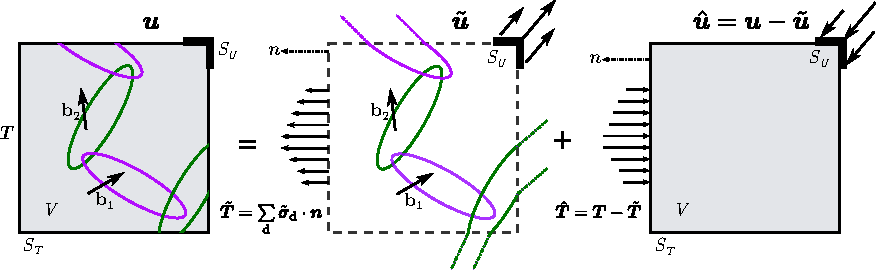
\includegraphics[width=\linewidth]{fem_ddd.pdf}
			\caption[Coupling Discrete Dislocation Dynamics to Finite Element Methods.]{The \kwd{dl} ensemble in a volume $ V $ is bounded by surface $ S $. First, the traction field $ \sum_{\textrm{d}} \tns{\tilde{\sigma}}_{\textrm{d}} $ due to the \kwd{dl} ensemble is evaluated at the surface. Then, a traditional \kwd{fem} or \kwd{bem} calculates the image traction field $ \tns{\hat{\sigma}} \times \vec{n} $. Which is then fed back to the \kwd{ddd} problem to evolve the \kwd{dl} positions and repeat the cycle. Image edited from \cite{analytical_integration_of_the_forces_induced_by_dislocations_on_a_surface_element}.}
			\label{f:fem_ddd}
		\end{figure}
	\section{Extracting Surface Nodes}
		The \kwd{fem} coupler arranges the nodes starting on the $ xz $-plane where $ y = 0, \ldots, n \mathrm{d}y,~n\in \mathbb{N} $. However in order to couple \kwd{ddd} to \kwd{fem} we only require the surface nodes where displacements are not calculated. Because we're working with rectangular prisms, we can easily pick out the surface nodes using a search algorithm with a logical mask. MATLAB and Fortran provide vector intrinsics that allow one to do so. \Cref{f:fem_surf_nodes} illustrates only the surface nodes according to our implementation's node arrangement---which is the $ xz $-plane going from $ y = y_{\textrm{min}} \to y = y_{\textrm{max}} $.
		\begin{figure}
			\centering
			\begin{subfigure}[b]{0.45\linewidth}
				\centering
				\includegraphics[width=\linewidth]{fem_surf_nodes.pdf}
				\caption[Surface nodes of our \kwd{fe} model.]{Arrangement of the surface nodes of our \kwd{fe} model.}
				\label{f:fem_surf_nodes}
			\end{subfigure}
			~
			\begin{subfigure}[b]{0.45\linewidth}
				\centering
				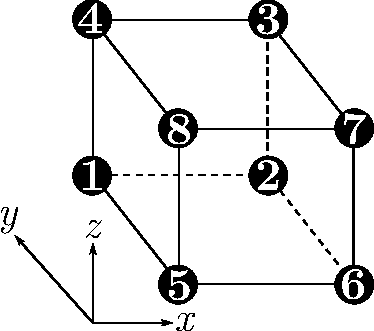
\includegraphics[width=\linewidth]{fe_numbering.pdf}
				\caption[Single finite element node numbering.]{Single \kwd{fe} node numbering.}
				\label{f:fe_numbering}
			\end{subfigure}
		\caption[Coupling Discrete Dislocation Dynamics to Finite Element Methods.]{Coupling Discrete Dislocation Dynamics to Finite Element Methods.}
		\label{f:fem_node_arr}
		\end{figure}
		However, due to the nature of the analytical solutions in \cref{c:lin_rect}, we need all the surface nodes of the rectangular faces for which there are no displacements. This means that edge nodes are shared between 2 adjacent faces and corner nodes between 3 adjacent faces. In order to properly apply the logical mask to find \emph{only} the surface nodes need to know that each \kwdp{fe}' nodes are numbered according to \cref{f:fe_numbering}.
		
		Using \cref{f:fem_node_arr} one can work out which nodes are of interest to whichever surface is being extracted. The ordering of the nodes in the final array will depend on the definition of the problems in \cref{c:lin_rect,c:quad_triang}.
		
		Node selection remains an expensive operation and minimising array indexing is of the utmost importance for the best perfomance. Selecting nodes in the traditional sense, i.e. with code branching such as \texttt{if statements} or \texttt{case selection} is unmantainable, verbose and very prone to mistakes. The issue was solved by introducing an auxiliary matrix which defines various parameters that aid node selection and greatly reduces code size, improves readability, and eliminates the need for code branching. The matrix can be constructed utilising \cref{f:fem_node_arr} in order to know which nodes correspond to which \kwd{fe} planes. The $ p\textsuperscript{th} $ column of the matrix\footnote{MATLAB uses column-major ordering, so this gives us the best performance for vectorised code.} corresponds to the $ p\textsuperscript{th} $ plane (according to an arbitrary plane numbering) and is defined as,
		\begin{align}\label{e:surf_node_util_vec}
			\vec{V_{p}}^{\mathsf{T}} =
				\begin{bmatrix}
					L_{1p} & L_{2p} & \cdots & L_{Np} & A_{p} & C_{p}
				\end{bmatrix}\,,
		\end{align}	
		where $ L_{np} $ is the numeric label for node $ n $ as given by \cref{f:fem_node_arr}, $ A_{p} $ is the area of the plane, and $ C_{p} $ is the numeric label of the orthogonal coordinate to the plane $ C_{p} = 1, ~2, ~3 $ for the $ x, ~y, ~z $ coordinates respectively. $ A_{p} $ lets us segment our output and transitional arrays so that the only data being modified is that which corresponds to the correct plane and $ C_{p} $ lets us know which coordinate we must use in our selection criteria. Using our particular node labelling scheme (with dimensions $ \Delta x,~ \Delta y,~ \Delta z $ respectively in the $ x,~ y,~ z $ directions), the matrix is defined as,
		\begin{align}\label{e:surf_node_util}
			\mtx{V} = 
				\begin{bmatrix}
					5 & 2 & 6 & 1 & 5 & 4\\
					1 & 6 & 5 & 2 & 6 & 3\\
					8 & 3 & 7 & 4 & 1 & 8\\
					4 & 7 & 8 & 3 & 2 & 7\\
					\Delta y \Delta z & \Delta y \Delta z & \Delta x \Delta z & \Delta x \Delta z & \Delta x \Delta y & \Delta x \Delta y\\
					1 & 1 & 2 & 2 & 3 & 3
				\end{bmatrix}\,.
		\end{align}
		The information codified in \cref{e:surf_node_util} lets us index and process only the necessary columns to extract the surface nodes we're interested in. The advantage of this setup over a naïve implementation is that it can be relatively easily expanded, maintained, and is general enough that it lends itself to a variety of selection criteria. The columns from left to right (1 to 6) represent: 
		\begin{inparaenum}[{face} 1 $ \equiv $]
			\item $ \min(x),~ yz $-plane;
			\item $ \max(x),~ yz $-plane;
			\item $ \min(y),~ xz $-plane;
			\item $ \max(y),~ xz $-plane;
			\item $ \min(z),~ xy $-plane;
			\item $ \max(z),~ xy $-plane.
		\end{inparaenum} 
		
		It is important to make sure the nodes are extracted in a self consistent manner because the problem definitions in \cref{c:lin_rect,c:quad_triang} assume a specific node ordering. In particular, the labelling chirality must remain the same. This is due to the fact that the problems in \cref{c:lin_rect,c:quad_triang} utilise internal coordinates derived from a set of basis vectors, and scalar projections onto them. If the relationship between the vectors is kept, but the chirality is different (opposite) the calculated quantities will have the wrong sign. If however the relationship between the vectors is different to the problem formulation, the program will crash due to division by 0. Self-consistency was achieved by placing an imaginary observer inside the \kwd{fe} model facing the $ \min(x),~ yz $-plane (face 1) and rotating it to view all 6 planes according to \cref{f:surf_node_plane}.
		\begin{figure}
			\centering
			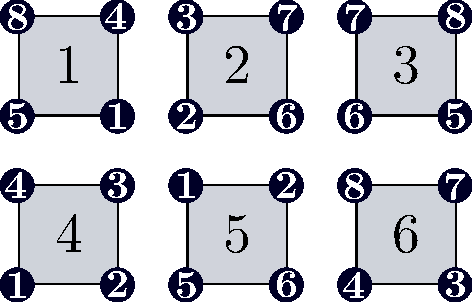
\includegraphics[width=0.75\linewidth]{surf_node_plane.pdf}
			\caption[Self-consistent, chirality preserving surface planes.]{Self-consistent, chirality preserving surface planes. Plane and node numbering according to the columns of \cref{e:surf_node_util} and \cref{f:fem_node_arr}.}
			\label{f:surf_node_plane}
		\end{figure}
		
		
	\chapter{Analytical Forces Induced by Dislocations on Linear Rectangular Surface Elements}
\label{c:lin_rect}
	%
	\section{Forces Exerted by a Dislocation Line Segment on Linear Rectangular Surface Elements}
	\label{s:f_lin_rect}
		%
		\begin{figure}
			\centering
			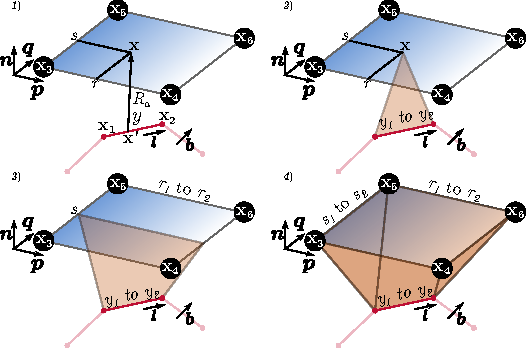
\includegraphics[width=\linewidth]{force_calc_linear_rectangle.pdf}
			\caption[Diagram of the analytical force calculation on linear rectangular surface elements.]{Diagram of the line integral method used to find analytical expressions for the forces exerted by \kwdp{dl} on linear rectangular \kwdp{se} \cite{analytical_integration_of_the_forces_induced_by_dislocations_on_a_surface_element}.
				\textit{1}) For any given point $ \vec{x} $ on the \kwd{se} and any given point $ \vec{x'}$ on the \kwd{dls}, define distance $ R_{a} $.
				\textit{2}) Integrate from $ x_{1} \to x_{2} $ along line direction $ \vec{t} $.
				\textit{3}) Integrate from $ r_{1} \to r_{2} $ along vector $ \vec{p} $.
				\textit{4}) Integrate from $ s_{1} \to s_{2} $ along vector $ \vec{q} $.}
			\label{f:flrs}
		\end{figure}
		\subsection{Resolving Singularities when Dislocation Line Segments are Parallel to Surface Elements}
		\label{ss:par_dln_se}
			%
			\begin{figure}
				\centering
				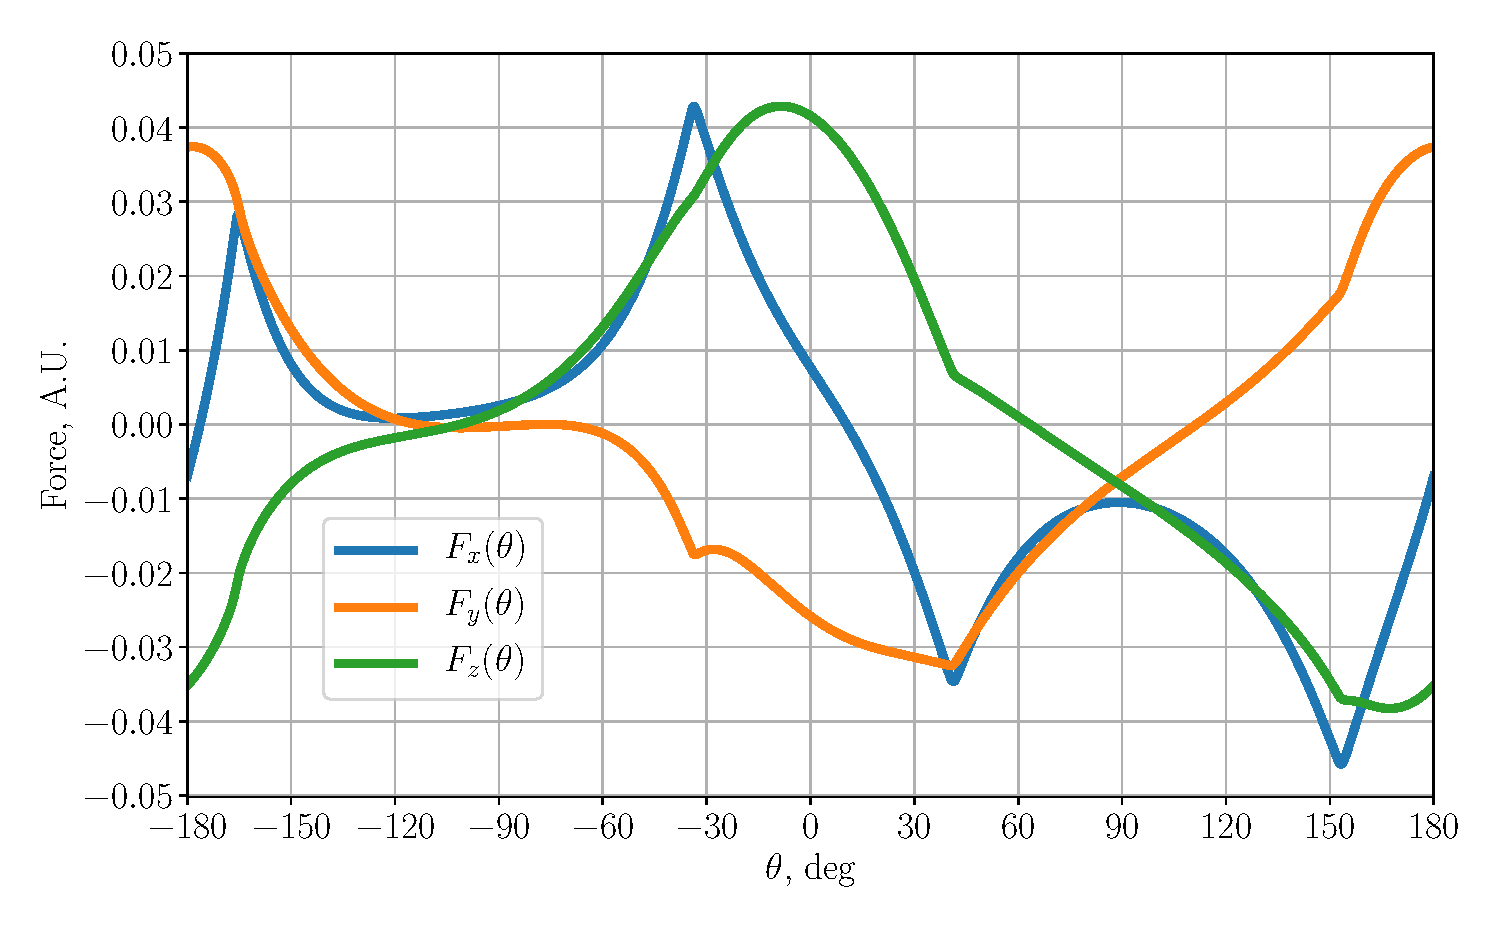
\includegraphics[width=\linewidth]{ftot_rotation_lin_rect.pdf}
				\caption[Avoiding singularities by rotating dislocation line segments.]{Effects of rotating a single \kwd{dls} on the forces exerted by it on a linear rectangular \kwd{se}. The specific values of this function are not known \emph{a priori}, all that is known is that it must be periodic ($ T = 2\pi$) and have finite maximum and minimum values. The singularity is avoided by perturbing the angle $ \theta = 0 \to \theta = \pm \epsilon\,\, \epsilon \gtrsim 0 $.}
				\label{f:rflrs}
			\end{figure}
		%
\savearabiccounter
	\chapter{Analytical Forces Induced by Dislocations on Quadratic Triangular Surface Elements}
\label{c:quad_triang}
	\section{Forces Exerted by a Dislocation Line Segment on Quadratic Triangular Surface Elements}
	\label{s:f_quad_triang}
	\begin{figure}
		\centering
		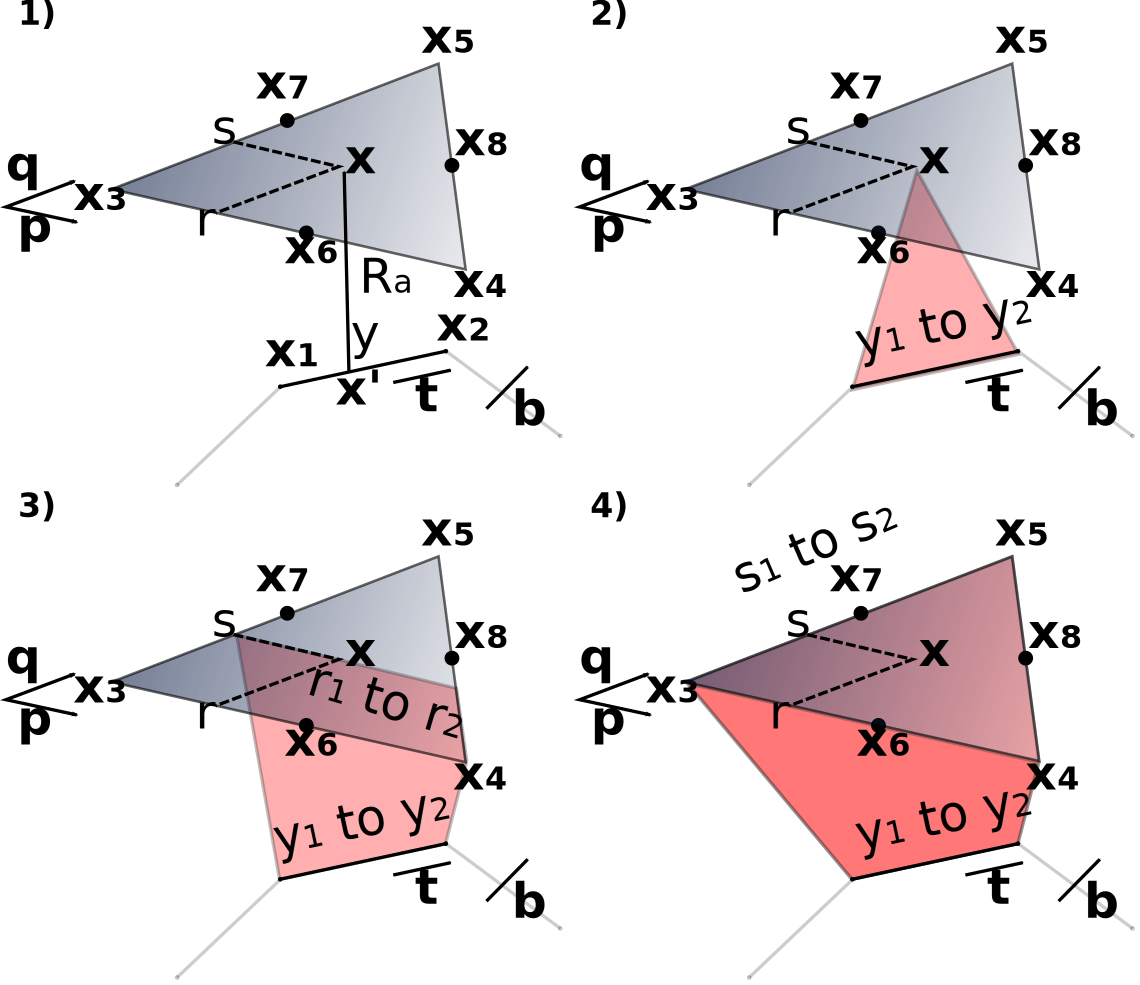
\includegraphics[width=\linewidth]{force_calc_quad_triangle.pdf}
		\caption[Diagram of the analytical force calculation on quadratic triangular surface elements.]{Diagram of the line integral method used to find analytical expressions for the forces exerted by \kwdp{dl} on quadratic triangular \kwdp{se}.}
		\label{f:fqts}
	\end{figure}
\savearabiccounter
	\chapter{Parallelisation of the Analytical Forces Induced by Dislocations on Surface Elements}
\label{c:para_f_dln_se}
	%
	\section{Parallelisation on Graphics Processing Units}
	Efficient parallelisation requires \kwd{cma}, which means we have to be extremely careful when mapping CPU memory to device memory. The fact that threads work ``simultaneously'' means that in order to obtain good performance, the data which is to be ``simultaneously'' loaded into each thread must be contiguous. This maximises cache memory use and therefore reduces slow memory fetch operations to global or shared memory.
	
	The parallelisation was done only over the \kwdp{se} in order to avoid the undesirable and inefficient GPU branching that would occur under other schemes.
	
	The most natural form of parallelisation is to have blocks of $ 4n $ threads where $ n \leq 8 \in \mathbb{N}$. This also fits nicely into the 32 thread per warp paradigm.
	%
	\subsection{Data Mapping}
		%
		\begin{figure}
			\centering
			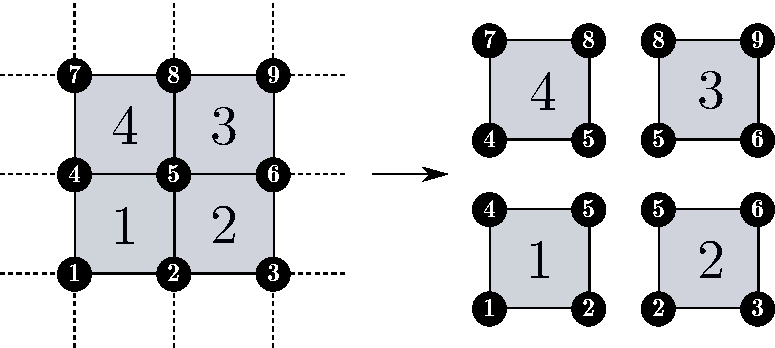
\includegraphics[width=\linewidth]{lrse_thread_map.pdf}
			\caption[Linear rectangular surface element mapping.]{Each linear rectangular \kwd{se} is mapped to one thread.}
			\label{f:lrse_map}
		\end{figure}
		%
		\subsubsection{Elements: Host $ \mapsto $ Device}
			%
			\begin{algorithm}
				\caption{Elements in host $ \mapsto $ device.}
				\label{a:ehd}
				\begin{algorithmic}[1]
					\Function{element\_host\_device\_map}{\hvar{\vec{X}[N][3\times E]}}
						\State{\Comment{Input, temporary, and output indices set to zero.}}
						\State{$ i,\, j,\, k \gets 0 $}
						\State{\Comment{\dvar{\vec{X}} accomodates all 3 coordinates of all $ N $ nodes in all $ E $ elements.}}
						\State{$ \dvar{\vec{X}} \gets $ malloc($ 3\times E\times N $)}
						\For{$(n = 0;\, n < N;\, n++)$} \Comment{Loop over nodes in element.}
							\State{\Comment{Set output index to point at the $ n\textsuperscript{th} $ node of the first coordinate of the first element.}}
							\State{$ k \gets j $}
							\For{$ (c = 0;\, c < 3;\, c++) $} \Comment{Loop over coordinates.}
								\State{\Comment{Set input index to point at the $ c\textsuperscript{th} $ coordinate of the first element of the $ n\textsuperscript{th} $ node.}}
								\State{$ i \gets c $}
								\For{$ (e = 0;\, e < E;\, e++) $} \Comment{Loop over elements.}
									\State{$ \dvar{\vec{X}[k + e]} \gets \hvar{\vec{X}[n][i]} $}
									\State{\Comment{Advance output index to point at the $ n\textsuperscript{th} $ node of the $ c\textsuperscript{th} $ coordinate of the first element.}}
									\State{$ i \gets i + 3 $}
								\EndFor
								\State{\Comment{Advance output index to point at the $ n\textsuperscript{th} $ node of the $ c\textsuperscript{th} $ coordinate of the first element.}}
								\State{$ k \gets k + E \times N $}
							\EndFor
							\State{\Comment{Advance temporary index to point at the $ (n+1)\textsuperscript{th} $ node of the first coordinate of the first element.}}
							\State{$ j \gets j + E $}
						\EndFor
						\State{\Return{\dvar{\vec{X}}}}
					\EndFunction
				\end{algorithmic}
			\end{algorithm}
		\subsubsection{Elements: Device $ \mapsto $ Thread}
			\begin{algorithm}
				\caption{Elements in device $ \mapsto $ thread.}
				\label{a:edt}
				\begin{algorithmic}[1]
						\GPUFunction[element\_device\_thread\_map]{\dvar{\vec{X}[3\times E\times N]}, \tvar{\vec{X}[N][3]}}
						\State{\Comment{Thread, input indices.}}
						\State{$ \rvar{idx},\, i \gets \rvar{threadIdx}.x + \rvar{blockIdx}.x\times \rvar{blockDim}.x $}
						\For{$ (n = 0;\, n < N;\, n++) $}\Comment{Loop over nodes in element.}
							\For{$ (c = 0;\, c < 3;\, c++) $}\Comment{Loop over elements.}
								\State{$ \tvar{\vec{X}[n][c]} \gets \dvar{\vec{X}[i + c\times E\times N]}$}
							\EndFor
							\State{$ i \gets i + E $}
							\Comment{Advance input index to the $(n+1)\textsuperscript{th}$ node of element $i$.}
						\EndFor
						\State{\Return{\tvar{\vec{X}[n][c]}}}
					\EndGPUFunction
				\end{algorithmic}    	
			\end{algorithm}
		\subsubsection{Force: Thread $ \xmapsto{+} $ Device}
			\begin{algorithm}
				\caption{Force in thread $ \xmapsto{+} $ device.}
				\begin{algorithmic}[1]
						\GPUFunction[add\_force\_thread\_device]{\tvar{\vec{F_{n}}[N][3]}, \tvar{\vec{F_{e}}[3]}, \dvar{\vec{F_{n}}[3\times E\times N]},\newline{}\dvar{\vec{F_{e}}[3\times E]}, \rvar{idx}}
						\State{\Comment{Nodal force.}}
						\State{\Comment{Set output index to whatever parallelisation index is given to the function. In this case the same index we use for the main parallelisation.}}
						\State{$ i \gets \rvar{idx} $}
						\For{$ (n = 0;\, n < N;\, n++) $} \Comment{Loop over nodes.}
							\For{$ (c = 0;\, c < 3;\, c++) $} \Comment{Loop over coordinates.}
								\State{\Comment{Ensure nodal forces are correctly added and mapped from local thread memory to global device memory.}}
								\State{atomicAdd(\dvar{\vec{F_{n}}[i + c\times E\times N]}, \tvar{\vec{F_{n}}[n][c]})}
							\EndFor
							\State{\Comment{Displace output index to point at the first coordinate of the $ (n+1)\textsuperscript{th} $ node of the \rvar{idx}\textsuperscript{th} \kwd{se}.}}
							\State{$ i \gets i + E $}
						\EndFor
						\State{\Comment{Total force.}}	
						\State{$ i \gets \rvar{idx} $} \Comment{Reset output index.}
						\For{$ (c = 0;\, c < 3;\, c++) $} \Comment{Loop over coordinates.}
							\State{atomicAdd(\dvar{\vec{F_{e}}[i]}, \tvar{\vec{F_{e}}[c]})}
							\State{\Comment{Advance the output index to point at the $ (i+1)\textsuperscript{th} $ coordinate of the $ \rvar{idx}\textsuperscript{th} $ \kwd{se}.}}
							\State{$ i \gets i + E $}
						\EndFor
						\State{\Return{\dvar{\vec{F_{n}}}, \dvar{\vec{F_{e}}}}}
					\EndGPUFunction
				\end{algorithmic}
			\end{algorithm}
		\subsubsection{Force (Parallelise over Dislocations): Thread $ \xmapsto{+} $ Device}
			\begin{algorithm}
				\caption{Force (parallelise over dislocations) in thread $ \xmapsto{+} $ device.}
				\begin{algorithmic}[1]
					\GPUFunction[dln\_add\_force\_thread\_device]{\tvar{\vec{F_{n}}[N][3]}, \tvar{\vec{F_{e}}[3]},\newline{}\dvar{\vec{F_{n}}[3\times E\times N]}, \dvar{\vec{F_{e}}[3\times E]}, $ k $}
						\State{\Comment{Nodal force.}}
						\State{\Comment{Set output index to correspond to whatever \kwd{se} we're on. By parallelising over dislocation lines, we must loop through \kwdp{se} in the main code, this is the value of $ k $ we provide. Multiply by 3 and $ N $ because each \kwd{se} has 3 coordinates and $ N $ nodes.}}
						\State{$ i \gets 3\times N\times k $}
						\State{$ j \gets 0 $} \Comment{Auxiliary index.}
						\For{$ (n = 0;\, n < N;\, n++) $} \Comment{Loop over nodes.}
							\For{$ (c = 0;\, c < 3;\, c++) $} \Comment{Loop over coordinates.}
								\State{\Comment{Ensure nodal forces are correctly added and mapped from local thread memory to global device memory.}}
								\State{atomicAdd(\dvar{\vec{F_{n}}[i + j + c]}, \tvar{\vec{F_{n}}[n][c]})}
							\EndFor
							\State{\Comment{Displace auxiliary index to point at the first coordinate of the $ (n+1)\textsuperscript{th} $ node of the $ k \textsuperscript{th}$ \kwd{se}.}}
							\State{$ j \gets j + 3 $}
						\EndFor
						\State{\Comment{Total force.}}
						\State{\Comment{Set auxiliary index to point at the first coordinate of the $ k\textsuperscript{th} $ \kwd{se}.}}
						\State{$ j \gets 3\times k $}
						\For{$ (c = 0;\, c < 3;\, c++) $} \Comment{Loop over coordinates.}
							\State{atomicAdd(\dvar{\vec{F_{e}}[j+c]}, \tvar{\vec{F_{e}}[c]})}
						\EndFor
						\State{\Return{\dvar{\vec{F_{n}}}, \dvar{\vec{F_{e}}}}}
					\EndGPUFunction
				\end{algorithmic}
			\end{algorithm}
		\subsubsection{Nodal Force: Device $ \mapsto $ Host}
			\begin{algorithm}
				\caption{Nodal force in device $ \mapsto $ host.}
				\begin{algorithmic}[1]
					\Function{fx\_device\_host\_map}{\dvar{\vec{F_{n}}[3\times E\times N]}, \hvar{\vec{F_{n}}[N][3\times E]}}
						\State{$ i,~j \gets 0 $} \Comment{Set input and output indices to zero.}
						\For{$ n = 0;\, n < N;\, n++ $} \Comment{Loop over nodes.}
							\State{$ j \gets 0 $} \Comment{Reset output index to point at the first element.}
							\For{$ e = 0;\, e < E;\, e++ $} \Comment{Loop over elements.}
								\For{$ c = 0;\, c < 3;\, c++ $} \Comment{Loop over coordinates.}
									\State{$ \hvar{\vec{F_{n}}[n][j + c]} = \dvar{\vec{F_{n}}[i + e + c\times E\times N]} $}
								\EndFor
								\State{\Comment{Advance output index to point at the first coordinate of the $ (e+1)\textsuperscript{th} $ element.}}
								\State{$ j \gets j + 3 $}
							\EndFor
							\State{\Comment{Advance input index to point at the first coordinate of the $ (n+1)\textsuperscript{th} $ node of the first element.}}
							\State{$ i \gets i + E $}
						\EndFor
						\State{\Return{\hvar{\vec{F_{n}}}}}
					\EndFunction
				\end{algorithmic}
			\end{algorithm}
		\subsubsection{Total Force: Device $ \mapsto $ Host}
			\begin{algorithm}
				\caption{Total force in device $ \mapsto $ host.}
				\begin{algorithmic}[1]
					\Function{ftot\_device\_host\_map}{\dvar{\vec{F_{e}}[3\times E]}, \hvar{\vec{F_{e}}[3\times E]}}
						\State{$ i \gets 0 $} \Comment{Set output index to zero.}
						\For{$ e = 0;\, e < E;\, e++ $} \Comment{Loop over elements.}
							\For{$ c = 0;\, c < 3;\, c++ $} \Comment{Loop over coordinates.}
								\State{$ \hvar{\vec{F_{e}}[i + c]} = \dvar{\vec{F_{e}}[e + c\times E]} $}
							\EndFor
							\State{\Comment{Advance the output index to point at the first coordinate of the $ (e+1)\textsuperscript{th} $ surface element.}}
							\State{$ i \gets i + 3 $}
						\EndFor
						\State{\Return{\hvar{\vec{F_{e}}}}}
					\EndFunction
				\end{algorithmic}
			\end{algorithm}
	\begin{subequations}\label{e:fcne}
		\begin{align}
			\vec{X}_{en}			&\coloneqq	\left[x_{en},\, y_{en},\, z_{en}\right]\\
			\vec{X}_{(1\to E)n}		&\mapsto 	\vec{X}_{n} \nn
			\vec{X}_{n}				&\coloneqq	\left[x_{1n},\, y_{1n},\, z_{1n},\ldots,x_{En},\, y_{En},\, z_{En}\right]\label{se:xn_arr}\\
			\vec{X}_{1\to N}		&\mapsto	\vec{X}^{\textrm{SE}}\nn
			\vec{X}^{\textrm{SE}}	&\coloneqq 
			\begin{aligned}
				&\left[x_{11},\, \ldots,\, x_{E1},\, x_{12},\, \ldots,\, x_{E2},\, \ldots,\, x_{1N},\, \ldots,\, x_{EN}, \right.\\
				&\left.\,y_{11},\, \ldots,\, y_{E1},\, y_{12},\, \ldots,\, y_{E2},\, \ldots,\, y_{1N},\, \ldots,\, y_{EN}, \right.\\
				&\left.\,z_{11},\, \ldots,\, z_{E1},\, z_{12},\, \ldots,\, z_{E2},\, \ldots,\, z_{1N},\, \ldots,\, z_{EN}  \right]
			\end{aligned}
		\end{align}
	\end{subequations}
	where $ e\equiv $~\kwd{se} label, $ n \equiv $~node label, $ E \equiv $~number of \kwdp{se} in the scope. $ N \equiv $~number of nodes in a \kwd{se}.
	
	Data-mapping according to \cref{a:fcne} and relabelling the nodes so they go from $ 0 \to N-1 $, the data from \cref{f:lrse_map} would be arranged in \kwd{devmem} like \cref{e:fcne_eg},
	\begin{align}\label{e:fcne_eg}
		\vec{X}^{\textrm{SE}} &= \begin{aligned}
			\left[\underbrace{h_{x},\, i_{x},\, f_{x},\, g_{x}}_{\mathbf{x_{0}}},\, 
			\underbrace{a_{x},\, b_{x},\, i_{x},\, h_{x}}_{\mathbf{x_{1}}},\, 
			\right.&\underbrace{i_{x},\, d_{x},\, e_{x},\, f_{x}}_{\mathbf{x_{2}}},\, 
			\underbrace{b_{x},\, c_{x},\, d_{x},\, i_{x}}_{\mathbf{x_{3}}},\\
			\ldots~y&\textrm{-coord}~\ldots,\\
			\ldots~z&\textrm{-coord}~\ldots]
		\end{aligned}
	\end{align}
	%
	
	In the GPU, each thread will cater to one \kwd{se} at a time. This means that each thread will have to extract the relevant data from the 1D array with length $ 3\times E\times N $ into four 1D arrays of length $ 3 $. The purpose of CNE mapping is to provide the \kwd{wrp} with \kwd{cma}. This is achieved via \cref{a:bcne}.
	
	
	Since \cref{a:bcne} is performed in a CUDA GPU, threads in a single block execute sequentially from,
	\begin{align}
		\rvar{threadIdx}.x &= 0 \to \rvar{threadIdx}.x = \rvar{blockDim}.x - 1\,,
	\end{align}
	while threads in different blocks execute in parallel. \Kwd{cma} is ensured by having each block load a cache line whose entries are contiguously accessed by the threads in the block. Using the same notation as \cref{a:fcne}, full cache line utilisation (optimal cache use) is achieved if cache lines can accomodate $ l $ entries given by \cref{e:opt_cache_len_bcne},
	\begin{align}
		\label{e:opt_cache_len_bcne}
		l =
		\begin{cases}
			a \times N \times E &,\, a > 0 \in \mathbb{N}\\
			&\textrm{or}\\
			\dfrac{1}{2^{a}} \times N \times E &,\, a \geq 0 \in \mathbb{N},\, N \times E \equiv 0\; (\bmod\; 2^{a})\,.
		\end{cases}
	\end{align}
	\Cref{f:fcne_eg} shows an example of \cref{a:bcne} up to the $ y $-coordinate.
	\begin{figure}
		\centering
		\includegraphics[width=\linewidth]{node_bmap.pdf}
		\caption[Example of the backward coodinate-node-element-map.]{Minimum working complete example of the backward coodinate-node-element-map. The explicit calculations of global indices correspond to subsituting the values for ``idx'' and ``idxi'' as in \cref{a:bcne}. $\vec{X_{a}^{b}}$ denotes a 1D array of length three containing the $ xyz $-coordinates of node $ a $ of element $ b $. Each thread concerns itself with only one element at a time. The dash-dot and dashed boxes represent cache lines for a thread block, the dotted line represents a memory fetch, and the dashed lines in $ \vec{X^{E}} $ represent steps of $ E $ entries (the start of the data for the next node of the element type we're dealing with). The memory operations are not shown twice to minimuse redundancy.}
		\label{f:fcne_eg}
	\end{figure}
	% Start: Code for generating figure e:opt_cache_len_bcne
	%\begin{align}%\label{f:fcne_eg}
	%	\vec{X}^{\textrm{SE}} &= 
	%							\begin{aligned}
	%								\left[\overbrace{h_{x},\, i_{x},\, f_{x},\, g_{x}}^{\mathbf{x_{3}}},\, 
	%								\overbrace{a_{x},\, b_{x},\, i_{x},\, h_{x}}^{\mathbf{x_{4}}},\, 
	%								\right.&\overbrace{i_{x},\, d_{x},\, e_{x},\, f_{x}}^{\mathbf{x_{5}}},\, 
	%								\overbrace{b_{x},\, c_{x},\, d_{x},\, i_{x}}^{\mathbf{x_{6}}},\\
	%								\overbrace{h_{y},\, i_{y},\, f_{y},\, g_{y}}^{\mathbf{x_{3}}},\, 
	%								\overbrace{a_{y},\, b_{y},\, i_{y},\, h_{y}}^{\mathbf{x_{4}}},\, 
	%								&\overbrace{i_{y},\, d_{y},\, e_{y},\, f_{y}}^{\mathbf{x_{5}}},\, 
	%								\overbrace{b_{y},\, c_{y},\, d_{y},\, i_{y}}^{\mathbf{x_{6}}},\\
	%								\overbrace{h_{z},\, i_{z},\, f_{z},\, g_{z}}^{\mathbf{x_{3}}},\, 
	%								\overbrace{a_{z},\, b_{z},\, i_{z},\, h_{z}}^{\mathbf{x_{4}}},\, 
	%								&\left.\overbrace{i_{z},\, d_{z},\, e_{z},\, f_{z}}^{\mathbf{x_{5}}},\, 
	%								\overbrace{b_{z},\, c_{z},\, d_{z},\, i_{z}}^{\mathbf{x_{6}}}\right]
	%\end{align}
	%\begin{align}
	%	\textrm{Parallel execution}
	%		&\begin{cases}
	%			&\vectorsym{X_{0}^{0}}[0] \gets \vectorsym{X^{E}}[(0+0\times 2) + (0\times 4 \times 4) + (0\times 4)]\nonumber\\
	%			&\vectorsym{X_{0}^{1}}[0] \gets \vectorsym{X^{E}}[(1+0\times 2) + (0\times 4 \times 4) + (0\times 4)]\nonumber\\
	%		\end{cases}\nonumber\\
	%	\textrm{Parallel execution}
	%		&\begin{cases}
	%			&\vectorsym{X_{0}^{2}}[0] \gets \vectorsym{X^{E}}[(0+1\times 2) + (0\times 4 \times 4) + (0\times 4)]\nonumber\\
	%			&\vectorsym{X_{0}^{3}}[0] \gets \vectorsym{X^{E}}[(1+1\times 2) + (0\times 4 \times 4) + (0\times 4)]\nonumber\\
	%		\end{cases}\nonumber\\
	%	\textrm{Parallel execution}
	%		&\begin{cases}
	%			&\vectorsym{X_{2}^{0}}[0] \gets \vectorsym{X^{E}}[(0+0\times 2) + (0\times 4 \times 4) + (2\times 4)]\nonumber\\
	%			&\vectorsym{X_{2}^{1}}[0] \gets \vectorsym{X^{E}}[(1+0\times 2) + (0\times 4 \times 4) + (2\times 4)]\nonumber\\
	%		\end{cases}\nonumber\\
	%	\textrm{Parallel execution}
	%		&\begin{cases}
	%			&\vectorsym{X_{2}^{2}}[0] \gets \vectorsym{X^{E}}[(0+1\times 2) + (0\times 4 \times 4) + (2\times 4)]\nonumber\\
	%			&\vectorsym{X_{2}^{3}}[0] \gets \vectorsym{X^{E}}[(1+1\times 2) + (0\times 4 \times 4) + (2\times 4)]\nonumber\\
	%		\end{cases}\nonumber\\
	%	%					
	%	\textrm{Parallel execution}
	%		&\begin{cases}
	%			&\vectorsym{X_{0}^{0}}[1] \gets \vectorsym{X^{E}}[(0+0\times 2) + (1\times 4 \times 4) + (0\times 4)]\nonumber\\
	%			&\vectorsym{X_{0}^{1}}[1] \gets \vectorsym{X^{E}}[(1+0\times 2) + (1\times 4 \times 4) + (0\times 4)]\nonumber\\
	%		\end{cases}\nonumber\\
	%	\textrm{Parallel execution}
	%		&\begin{cases}
	%			&\vectorsym{X_{0}^{2}}[1] \gets \vectorsym{X^{E}}[(0+1\times 2) + (1\times 4 \times 4) + (0\times 4)]\nonumber\\
	%			&\vectorsym{X_{0}^{3}}[1] \gets \vectorsym{X^{E}}[(1+1\times 2) + (1\times 4 \times 4) + (0\times 4)]\nonumber\\
	%		\end{cases}\nonumber\\
	%	\textrm{Parallel execution}
	%		&\begin{cases}
	%			&\vectorsym{X_{2}^{0}}[1] \gets \vectorsym{X^{E}}[(0+0\times 2) + (1\times 4 \times 4) + (2\times 4)]\nonumber\\
	%			&\vectorsym{X_{2}^{1}}[1] \gets \vectorsym{X^{E}}[(1+0\times 2) + (1\times 4 \times 4) + (2\times 4)]\nonumber\\
	%		\end{cases}\nonumber\\
	%	\textrm{Parallel execution}
	%		&\begin{cases}
	%			&\vectorsym{X_{2}^{2}}[1] \gets \vectorsym{X^{E}}[(0+1\times 2) + (1\times 4 \times 4) + (2\times 4)]\nonumber\\
	%			&\vectorsym{X_{2}^{3}}[1] \gets \vectorsym{X^{E}}[(1+1\times 2) + (1\times 4 \times 4) + (2\times 4)]\nonumber\\
	%		\end{cases}\nonumber
	%\end{align}
	% End: Code for generating figure e:opt_cache_len_bcne
	\subsubsection{Node Coordinate Element Map}
	%
	The node-coordinate-element (NCE) data mapping in \cref{e:fnce} is carried out by \cref{a:fnce}, each thread looks after a given \kwd{se}.
	\begin{algorithm}
		\caption{NCE data mapping.}
		\label{a:fnce}
		\begin{algorithmic}
			\ForAll{n nodes $ \in $ surface element}
			\ForAll{c coordinates $ \in [x,\, y,\, z] $}
			\ForAll{e surface elements $ \in $ surface mesh section}
			\State list.append(data of the $ n\textsuperscript{th}$ node with $ c\textsuperscript{th} $ coordinate of the $ e\textsuperscript{th} $ SE)
			\EndFor
			\EndFor
			\EndFor
		\end{algorithmic}
	\end{algorithm}
	\begin{subequations}\label{e:fnce}
		\begin{align}
			\vec{X}_{en}			&\coloneqq \left[x_{en},\, y_{en},\, z_{en}\right]\\
			\vec{X}_{(1\to E)n}		&\mapsto \vec{X}_{n} \nn
			\vec{X}_{n}				&\coloneqq \left[x_{1n},\ldots,\, x_{En},\, y_{1n},\ldots,\, y_{En},\, z_{1n},\ldots,\, z_{En}\right]\\
			\vec{X}_{1\to N}		&\mapsto \vec{X}^{\textrm{SE}}\nn
			\vec{X}^{\textrm{SE}}	&\coloneqq 
			\begin{aligned}
				\left[x_{11},\ldots,\, x_{E1},\, y_{11},\right.&\ldots,\, y_{E1},\, z_{11},\ldots,\, z_{E1}\\
				,&\ldots,\\
				x_{1M},\ldots,\, x_{EN},\, y_{1N},&\left.\ldots,\, y_{EN},\, z_{1N},\ldots,\, z_{EN}\right]
			\end{aligned}
		\end{align}
	\end{subequations}
	where $ e\equiv $~surface \textbf{e}lement, $ n \equiv $~\textbf{n}ode, $ E \equiv $~total number of \kwdp{se} in scope, $ N \equiv $~total number of nodes in each \kwd{se}.
	
	Data-mapping according to \cref{a:fnce} and relabelling the nodes so they go from $ 0 \to N-1 $, the data from \cref{f:lrse_map} would be arranged in \kwd{devmem} like \cref{e:fnce_eg},
	\begin{align}\label{e:fnce_eg}
		\vec{X}^{\textrm{SE}} &= \begin{aligned}
			&\left[\underbrace{h_{x},\, i_{x},\, f_{x},\, g_{x},\, 
				h_{y},\, i_{y},\, f_{y},\, g_{y},\, 
				h_{z},\, i_{z},\, f_{z},\, g_{z}}_{\mathbf{x_{0}}}\right.,\\
			&~\ldots~\mathbf{x_{1}},\, xyz\textrm{-coords}~\ldots,\\
			&~\ldots~\mathbf{x_{2}},\, xyz\textrm{-coords}~\ldots,\\
			&~\ldots~\mathbf{x_{3}},\, xyz\textrm{-coords}~\ldots]
		\end{aligned}
	\end{align}
	%
	\subsubsection{Resolving Data Write Conflicts}
	Data write conflicts can be a problem in parallel applications where global data is changed by multiple threads within the same clock tick. This can be avoided with \kwdp{atop}.
	%
	\subsection[Parallel Dislocation Line Segments to Surface Elements]{Resolving Parallel Dislocation Line Segments to Surface Elements}
	%
	Dealing with the special case when the \kwd{dls} $ \vec{t} $ is parallel to the \kwd{se} is relatively trivial when in a serial program. By the mean value theorem, we can slightly perturb $ \vec{t} $ by rotating it by a small angle around the midpoint of $ \vec{t} $ with respect to the axis of rotation defined by $ \vec{t} \times \vec{n} $. In contrast to serial code, program branches can have a serious effect on parallel performance due to \kwd{wrpd}. Due to the complexity of the force calculation and relative rarity of the edge case, there is no branching behaviour in the parallel code until \emph{after} the calculation is performed. Where \cref{a:plse_p} is performed.
	\begin{algorithm}
		\caption{Resolving cases when $ \vec{t} \parallel \vec{n} $ on GPUs.}
		\label{a:plse_p}
		\begin{algorithmic}
			\ForAll{surface elements \emph{and} line segments}
			\State $ \ldots $
			\If{$ \vec{t}_{\textrm{thread}} \parallel \vec{n}_{\textrm{thread}} $}
			\State $ \vec{x}_{\textrm{buffer}} \gets \vec{x}_{\textrm{thread}} $
			\State $ \vec{t}_{\textrm{buffer}} \gets \vec{t}_{\textrm{thread}} $
			\Else
			\State $ \vec{F}_{\textrm{total}} += \vec{F}_{\textrm{thread}} $
			\EndIf
			\EndFor
			\State return to serial code
			\If{$ \vec{x}_{\textrm{buffer}} \neq $ empty}
			\ForAll{surface elements \emph{and} line segments}
			\State perform calculation for $ \vec{t} \parallel \vec{n} $
			\EndFor
			\EndIf
		\end{algorithmic}
	\end{algorithm}
	\subsubsection{Implementation}
	The node mapping would be the same as \cref{a:fcne}. The parallelisation would be on individual packets of a \kwd{se} with a slightly rotated \kwd{dls}, as in a single iteration of the serial code where the \kwd{dls} is rotated. The forces would be averaged with \kwdp{atop} and \mintinline{c}{__syncthreads()} before they are added to the total nodal forces.
	
	\subsection{Test Case}
	\begin{figure}
		\includegraphics[width=\linewidth]{cuda_test.pdf}
		\caption[Test case for CUDA development.]{Test case for CUDA development. Dislocation line not shown in node separation as the parallelisation happens across surface elements. Not to perspective or scale.}
		\label{f:cuda_test}
	\end{figure}
	According to \cref{a:fcne} and the node labelling scheme of \cref{f:flrs} the data mapping would look like:
	\begin{align}\label{e:cuda_test}
		\vec{X}^{\textrm{SE}} = 
		\begin{split}
			\left[\overbrace{\underbrace{1,1,0,0}_{\mathbf{x_{3}}}, \underbrace{2,2,1,1}_{\mathbf{x_{4}}},
				\underbrace{1,1,0,0}_{\mathbf{x_{5}}}, \underbrace{2,2,1,1}_{\mathbf{x_{6}}}}^{x\textrm{-coord}},\right.\\
			\overbrace{\underbrace{0,1,1,0}_{\mathbf{x_{3}}}, \underbrace{0,1,1,0}_{\mathbf{x_{4}}},
				\underbrace{1,2,2,1}_{\mathbf{x_{5}}}, \underbrace{1,2,2,1}_{\mathbf{x_{6}}}}^{y\textrm{-coord}},\\
			\left.\overbrace{\underbrace{0,0,0,0}_{\mathbf{x_{3}}}, \underbrace{0,0,0,0}_{\mathbf{x_{4}}},
				\underbrace{0,0,0,0}_{\mathbf{x_{5}}}, \underbrace{0,0,0,0}_{\mathbf{x_{6}}}}^{z\textrm{-coord}}\right]
		\end{split}
	\end{align}
	In general the number of indices in the array would be $ 3 \times e \times n $ where $ e \equiv $~number of surface elements, $ n \equiv $~number of nodes per element and 3 is the number of spatial dimensions.
	\savearabiccounter
	% References
	%\renewcommand{\bibname}{References} % Change bibliography name to References.
\bibliographystyle{unsrtnat}
\bibliography{bib}
\savearabiccounter
	% Appendices
	\appendix
	\chapter{Best Practices}\label{c:best_practices}
	This chapter defines the best practices that will make improve the development and testing pipeline by defining rules and standards that facilitate collaboration.
	\section{Filesystem}\label{c:best_practices:s:filesystem}
		All files must be within \texttt{/project\_name}. 
		\begin{enumerate}
			\item All files must be within \texttt{/project\_name},\\
				  \texttt{\textasciitilde/} = \texttt{project\_name/}, \\
				  \texttt{\textasciitilde/\textasciitilde/} = \texttt{project\_name/src/} or \texttt{project\_name/dev/}.
			\item Release code must be within \texttt{\textasciitilde/src/}.
			\item Development code must be within \texttt{\textasciitilde/dev/}.
			\item Test data must be within \texttt{\textasciitilde/tests/}.
			\item Documentation must be within \texttt{\textasciitilde/\textasciitilde/doc/}.
			\item Examples must be within \texttt{\textasciitilde/\textasciitilde/exmp/}.
			\item External libraries must be within \texttt{\textasciitilde/lib/}.
			\item Generated images must be within \texttt{\textasciitilde/\textasciitilde/images/}.
			\item Old versions recordkeeping must be within \texttt{\textasciitilde/prv/va.b.c/}.
		\end{enumerate}
	%
	\section{Versioning}\label{c:best_practices:s:versioning}
		\begin{enumerate}
			\item Use a version control system like \href{https://github.com/}{GitHub} or \href{https://pastebin.com/}{PasteBin}.
			\item There must be a master branch that is only changed when the code is stable and bug free.
			\item Development branches should be exploited as seen fit without making things overly convoluted.
			\item Commits must be as bug free and regular as possible. When to commit is left to the developer's discresion.
			\item Commit messages should be as descriptive as possible.
			\item Versions should be specified as \texttt{va.b.c} where \texttt{a}, \texttt{b}, \texttt{c} = integers. The three levels are \texttt{a} = release version (usable, bug free code), \texttt{b} = beta version (code that is undergoing testing), \texttt{c} = alpha version (code that is under active development).
		\end{enumerate}
	%	 
	\section{Documentation}\label{c:best_practices:s:documentation}
		\subsection{Commenting}\label{c:best_practices:s:documentation:ss:commenting}
			Every codefile must be appropriately commented by meeting the following guidelines.
			\begin{enumerate}
				\item The start of each codefile must have a heading detailing the creator, date of creation and edit history (date and name of editor).
				\item Below the heading there must be a general explanation of the code. It must state any procedures, structures, objects and how they are to be utilised. Any backward or forward dependencies must be stated.
				\item Below the description and edit history any relevant literature must be mentioned (dois are preferred). Must be as detailed as possible, include equation numbers/ranges if necessary.
				\item The start of every procedure has an explanation of its purpose, inputs, outputs and inputs-outputs.
				\item Particularly complicated code blocks must have an in-depth explanation of what it does. Comment each line if necessary.
				\item Corrections or additions must be explicitly bounded by comments at the start and end of the change. Both bounding comments must have the author's name and the date. Below the starting comment, there should be an explanation of the change. Any punctual comments can be made as normal.
			\end{enumerate}
		\subsection{README}\label{c:best_practices:s:documentation:ss:readme}
			Every codefile must have an associated \textsc{readme} \texttt{.tex} document that documents the codefile's contents. It must meet the following guidelines as appropriate.
			\begin{enumerate}
				\item The name must be that of the file it documents (minus the extension of course).
				\item Description and overall explanation of the codefile's purpose.
				\item Overall flow chart or pseudo code describing the file's purpose.
				\item Document the codefile's procedures. This means describing and explaining their corresponding inputs, outputs, inputs-outputs, forwards and backwards dependencies, and flow charts or pseudo codes.
				\item Unit test designs and results for each procedure. If appropriate also include those of integral tests.
			\end{enumerate}
			The codefile may also be appended at the end of documentation if desired (the \texttt{minted} package is highly recommended).
	%
	\section{Modularisation}\label{c:best_practices:s:modularisation}
		\begin{enumerate}
			\item Code repetition must be kept to a \emph{strict} minimum. Any piece of code that will be reused must be modularised.
			\item Procedures must be as self-sufficient as possible \emph{without} repeating code. If repeating code is necessary, replace it with a procedure that is to be repeatedly called instead. Minimising repeated code $\ggg$ procedure self-sufficiency.
		\end{enumerate}
	%
	\section{Coding Style}\label{c:best_practices:s:naming_conventions}
		All names must meet the following guidelines.
		\begin{enumerate}
			\item Indent appropriately. Four space tabs are a good compromise between code necking and readability.
			\item Minimise the use of nested code blocks, use intrisics, libraries or create procedures instead.
			\item Break up lines that are uncomfortably long, typically anything over 80--100 characters.
			\item Names should be appropriately descriptive and human readable.
			\item All code and names must be systematic and logical.
			\item the use of upper cases should be reserved for parameters (\texttt{const} variables in C).
			\item Delimit words with ``\texttt{\_}'' \emph{not} case changes.
			\item Long and descriptive $\ggg$ short and cryptic.
		\end{enumerate}
		\subsection{Filenames}\label{c:best_practices:s:naming_conventions:ss:filenames}
			\begin{enumerate}
				\item If old versions are to be kept, the old \emph{stable} versions of file must have the date of last modification appended \emph{suffixed} after the file extension in the \texttt{\_yyyymmdd} format. For example, if the stable version of the release code \texttt{hello\_world\_parallel.c} was last modified on April 25, 2017 it should be archived as\\ \texttt{hello\_world\_parallel.c\_20170425}.
			\end{enumerate}
		\subsection{Variables, Structures and Objects}\label{c:best_practices:s:naming_conventions:ss:variables_structures_objects}
			\begin{enumerate}
				\item Only counters and indices can be single letter variables.
				\item Structure and object \emph{definitions} are \emph{suffixed} with \texttt{\_s} and \texttt{\_o} respectively.
				\item Inputs, outputs and input-outputs to procedures must be \emph{prefixed} with \texttt{i\_}, \texttt{o\_} and \texttt{io\_} respectively.
			\end{enumerate}
		\subsection{Procedures}\label{c:best_practices:s:naming_conventions:ss:procedures}
			\begin{enumerate}
				\item Functions and subroutines must be \emph{prefixed} with \texttt{f\_} and \texttt{s\_} respectively.
			\end{enumerate}
	\chapter{Coupling Discrete Dislocation Dynamics to Finite Element Methods}

\inputminted[breaklines, linenos, fontsize=\normalsize]{matlab}{../EasyDD/extract_node_plane.m}

\inputminted[breaklines, linenos, fontsize=\normalsize]{matlab}{../EasyDD/extract_node_planes.m}

\inputminted[breaklines, linenos, fontsize=\normalsize]{matlab}{../EasyDD/analytic_traction.m}

	\chapter{Implementation of Analytical Forces Induced by Dislocations on Linear Rectangular Surface Elements}
	\section{Serial C Code MEX File}
	%\inputminted[breaklines, linenos, fontsize=\normalsize]{c}{../../../Dropbox/Daniel/DDLabFEM/nodalForce/nodal_surface_force_linear_rectangle_arr_unix.c}
	\section{Parallel CUDA C Code MEX File}
\savearabiccounter
		
	\chapter{Implementation of Analytical Forces Induced by Dislocations on Quadratic Triangular Surface Elements}
	\section{Serial C Code MEX File}
	%\inputminted[breaklines, linenos, fontsize=\normalsize]{c}{../../../Dropbox/Daniel/DDLabFEM/nodalForce/nodal_surface_force_quad_triangle_qp.c}
	\section{Parallel CUDA C Code MEX File}

	\chapter{Talks}
	\section{Durham July 12--14 2017}
		Bridging the gap between the microscopic and macroscopic world is an on-going challenge for science and technology. If we hope to understand complex emergent phenomena we need to study systems that blur the line between micro and macro. In materials science, one such area is the study of extended defects called dislocations; whose nucleation and movement mediate the permanent deformation of materials. These large, high energy defects present very complex and long ranged interactions with each other, crystal boundaries, impurities, free surfaces, and themselves. As such, their dynamics are difficult to study experimentally. So we make justified assumptions and simplifications and create models that let us study them in detail. However if our models are to prove useful in real applications, they must be continually refined and improved by weakening assumptions and removing simplifications. Unfortunately, with increased refinement comes increased computational cost and new challenges. Therefore, finding faster alternatives that do not sacrifice accuracy is of the utmost importance---better yet if the alternatives are more accurate or exact. With the advent of increasingly accessible graphics processor units (GPUs) typically used in video gaming, the power of parallel processing is no longer exclusive to researchers with access to supercomputers. In this talk we will discuss the GPU implementation of exact solutions for the forces dislocations exert on the surfaces of materials.
	% Backmatter
	\begin{romanpages}
	\printglossary[nonumberlist]
	\phantomsection
	\addcontentsline{toc}{chapter}{Index} % Add index to the table of contents (toc).
	\printindex
\end{romanpages}
\end{document}
